\documentclass[a4paper, 11pt]{article}
\usepackage{graphicx}
\usepackage{amsmath}
\usepackage{float}
\usepackage[inner=1in, top=1in, bottom=1in]{geometry}
\usepackage{amsfonts}
\usepackage{hyperref}
\usepackage{color,soul}

\DeclareMathOperator{\Cor}{Cor}
\DeclareMathOperator{\Cov}{Cov}
\DeclareMathOperator{\STD}{STD}
\DeclareMathOperator{\Var}{Var}
\DeclareMathOperator{\E}{E}
\DeclareMathOperator{\Tr}{Tr}
\DeclareMathOperator{\diag}{\text{diag}}
\DeclareMathOperator{\f}{\boldsymbol{f}}
\DeclareMathOperator{\x}{\boldsymbol{x}}
\DeclareMathOperator{\y}{\boldsymbol{y}}
\DeclareMathOperator{\z}{\boldsymbol{z}}
\DeclareMathOperator{\pa}{\boldsymbol{\theta}}


\begin{document}

\title{An Introduction to Gaussian Process Regression}
\author{P.L.Green\\
Institute for Risk and Uncertainty\\
School of Engineering\\
University of Liverpool\\
Liverpool, L69 7ZF\\
United Kingdom\\
\\
\href{mailto:p.l.green@liverpool.ac.uk}{p.l.green@liverpool.ac.uk} \\
\url{https://www.liverpool.ac.uk/engineering/staff/peter-green/}
}
\maketitle

\section{Introduction}
This document is supposed to provide a tutorial-style introduction to Gaussian Process (GP) regression. It comes with some example Gaussian Process code, written in Python, that is free and should be relatively easy to use. The code is by no-means optimised, rather, it is supposed to be easy to read and easy to understand for someone who is new to GP regression. 

\section{The Problem}
Say we believe that a system's input, $\x$, is related to its output via a relationship $f(\x)$. The function, $f$, is currently unknown. To help us find $f$, we conduct a series of experiments where, for $N$ different $\x$ values, we observe the system's output (denoted $y$). Our experiment therefore yields the data $(\x_1,y_1),...,(\x_N,y_N)$. As with any experiment, our observations are corrupted by some errors. In the following, we treat these errors as being Gaussian and we assume the following `noise model':

\begin{equation}
	y_i = f(\x_i) + \epsilon, \qquad \epsilon \sim \mathcal{N}(\epsilon;0,\sigma^2)
	\label{eq:noise_model}
\end{equation}
that is, we assume that each observation $y_i$ is equal to the function, $f$, evaluated at input, $\x_i$, but corrupted with Gaussian noise of variance $\sigma^2$. 

\section{Bayesian Linear Regression}
Once we have our data,  $(\x_1,y_1),...,(\x_N,y_N)$, we can use it to try and infer the function $f$. Say we assume that $f$ takes the form

\begin{equation}
	f(\x_i) = \pa^T \boldsymbol{\phi}(\x_i)
	\label{eq:linear_regression}
\end{equation}
where $\pa$ is a vector of parameters which we need to estimate and $\boldsymbol{\phi}$ is a `basis function'. For example, if we are considering univariate inputs and set

\begin{equation}
	\pa = (\theta_0,\theta_1,\theta_2)^T, \qquad \boldsymbol{\phi}(x_i) = (1,x_i,x_i^2)^T
\end{equation}
then we would be trying to fit a quadratic function to our data. Equation (\ref{eq:linear_regression}) is convenient because it is a linear function of the parameters we need to estimate - this usually makes it easier to find closed-form expression for the `optimum choice' of $\pa$. \\

Defining

\begin{equation}
	\f = ( f_1,f_2,...,f_N )^T,  \qquad \text{where} \qquad f_i \equiv f(\boldsymbol{x}_i) 
\end{equation}
we can write

\begin{equation}
	f_i = \sum_k \theta_k \phi_k(\boldsymbol{x}_i).
\end{equation}
Furthermore, defining the matrix

\begin{equation}
\boldsymbol{\Phi} =
\left[
  \begin{array}{ccc}
    \phi_1(\boldsymbol{x}_1) & \phi_2(\boldsymbol{x}_1) & ... \\
    \phi_1(\boldsymbol{x}_2) & \phi_2(\boldsymbol{x}_2) &  \\
    \vdots &  & \ddots \\
  \end{array}
\right]
\end{equation}
lets us write $\f=\boldsymbol{\Phi}\pa$. \\

At this point, a Bayesian approach would typically involve defining a prior probability distribution, $p(\pa)$, that is supposed to represent our prior belief in $\pa$. We would then write down Bayes theorem:

\begin{equation}
	p(\pa|\y) \propto p(\y|\pa)p(\pa)
\end{equation}
where $\y=(y_1,...,y_N)$ is our observation data and the likelihood, $p(\y|\pa)$, is formed based on our noise model (equation (\ref{eq:noise_model}) in this case). This approach gives us an expression for the posterior distribution, $p(\pa|\y)$, which allows us to analyse the probability that our regression parameters can take particular values, conditional on our observation data.\\

If we adopt such a Bayesian approach and happen choose the prior over our parameters to be

\begin{equation}
	p(\pa) = \mathcal{N}(\pa; \boldsymbol{0}, \alpha^{-1}\boldsymbol{I})
\end{equation}
then, after `feeding it through' our model ($\f=\boldsymbol{\Phi}\pa$), it follows that the covariance matrix over $\f$ is

\begin{equation}
	\Cov[\f] = \E[\f\f^T] = \boldsymbol{\Phi}\E[\pa\pa^T]\boldsymbol{\Phi}^T = \alpha^{-1}\boldsymbol{\Phi}\boldsymbol{\Phi}^T
\end{equation}
(which we'll write just as $\Cov[\boldsymbol{y}] = \boldsymbol{K}$ from now on). This result means that, regardless of the inputs used in our experiments, saying that our prior over $\pa$ is Gaussian means we automatically assume a Gaussian prior over $\f$:

\begin{equation}
	p(\f) \propto \exp\left( -\frac{1}{2} \f^T\boldsymbol{K}^{-1}\f \right).
\end{equation}
where the individual elements of $\boldsymbol{K}$ are given by

\begin{equation}
	K_{ij} = \alpha^{-1} \sum_i \phi_i(\boldsymbol{x}_i) \phi_i(\boldsymbol{x}_j) 
	\label{eq:linear_regression_K}
\end{equation}	
	
\section{Gaussian Process Regression}
In the previous section we defined a function $f$ that was linear in our regression parameters, $\pa$, before defining a Gaussian prior over $\pa$. This led to a Gaussian prior over $\f$, whose covariance matrix is given by equation (\ref{eq:linear_regression_K}). Key to the construction of GPs is the idea that, as we know that the aforementioned Bayesian approach will always lead to a Gaussian distribution over $\f$, we  may as well define $p(\f)$ directly and skip the part where we define a basis function and a prior over $\pa$. Specifically, we simply write

\begin{equation}
	p(\f) = \mathcal{N}(\f;\boldsymbol{0},\boldsymbol{K})
\end{equation} 
where the matrix $\boldsymbol{K}$ can be anything we like (so long as it is a valid covariance matrix). For this reason, GPs are sometimes described as a method that `assigns a prior over the function values, $\f$'. The matrix $\boldsymbol{K}$ (the `gram matrix') is usually defined using a \emph{kernel function}, $k$, such that $\boldsymbol{K}_{ij} = k(\x_i,\x_j)$. A common choice of kernel function, for example, is 

\begin{equation}
	k(\x_i,\x_j) = \exp \left( -\frac{1}{2 l^2} (\x_i-\x_j)^T(\x_i-\x_j) \right)
	\label{eq:typical_kernel_function}
\end{equation}
where we have introduced $l$, a `length scale' parameter. So how do the kernel function (equation (\ref{eq:typical_kernel_function})) and length scale parameter alter our prior belief about the function $f$? Consider the case where we have a vector of 100 1D inputs, that are evenly spaced between 0 and 10. We choose the kernel described by equation (\ref{eq:typical_kernel_function}) and plot the matrix $\boldsymbol{K}$ for $l=10,1$ and $0.1$. The resulting gram matrices are shown in Figure \ref{fig:K_lengthscales}.\\

\begin{figure}[H]
	\centering
	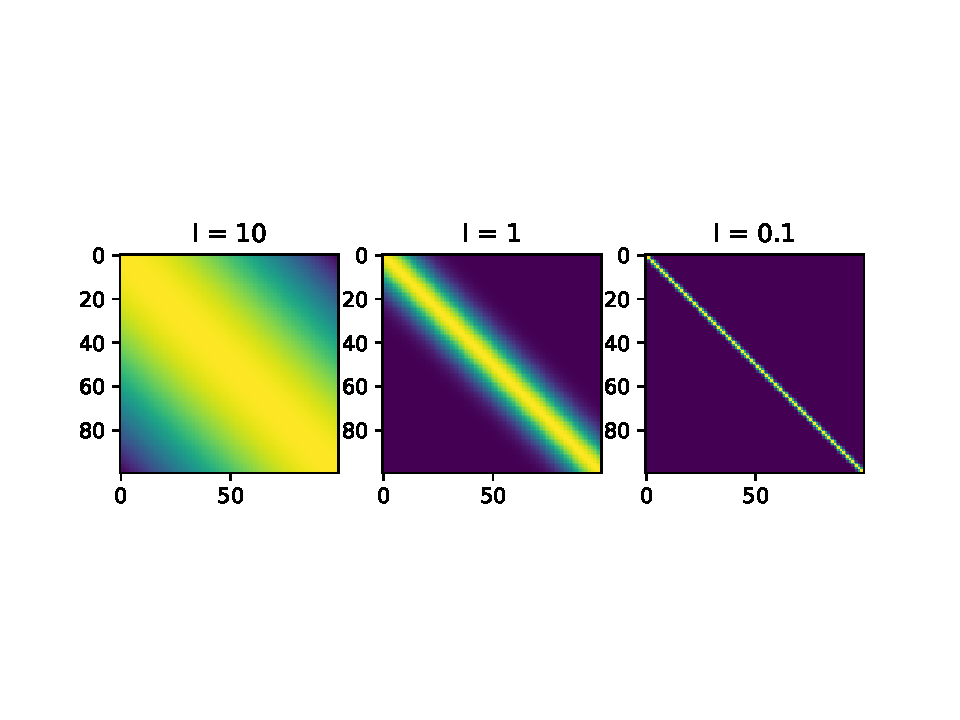
\includegraphics[scale=0.8,trim={0 2cm 0 2cm},clip]{figures/K_images.pdf}
	\caption{Plotting the gram matrix, $\boldsymbol{K}$, for different values of length scale, $l$, using the kernel function described by equation (\ref{eq:typical_kernel_function}).}
	\label{fig:K_lengthscales}
\end{figure}
Figure \ref{fig:K_lengthscales} shows us that, by using larger values of $l$, we are introducing greater correlation between our inputs. So what does this signify? Generating 100 samples of $\f$, from $\mathcal{N}(\f;\boldsymbol{0},\boldsymbol{K})$ for different values of $l$, we realise the results shown in Figure \ref{fig:prior_over_f}.\\

\begin{figure}[H]
	\centering
	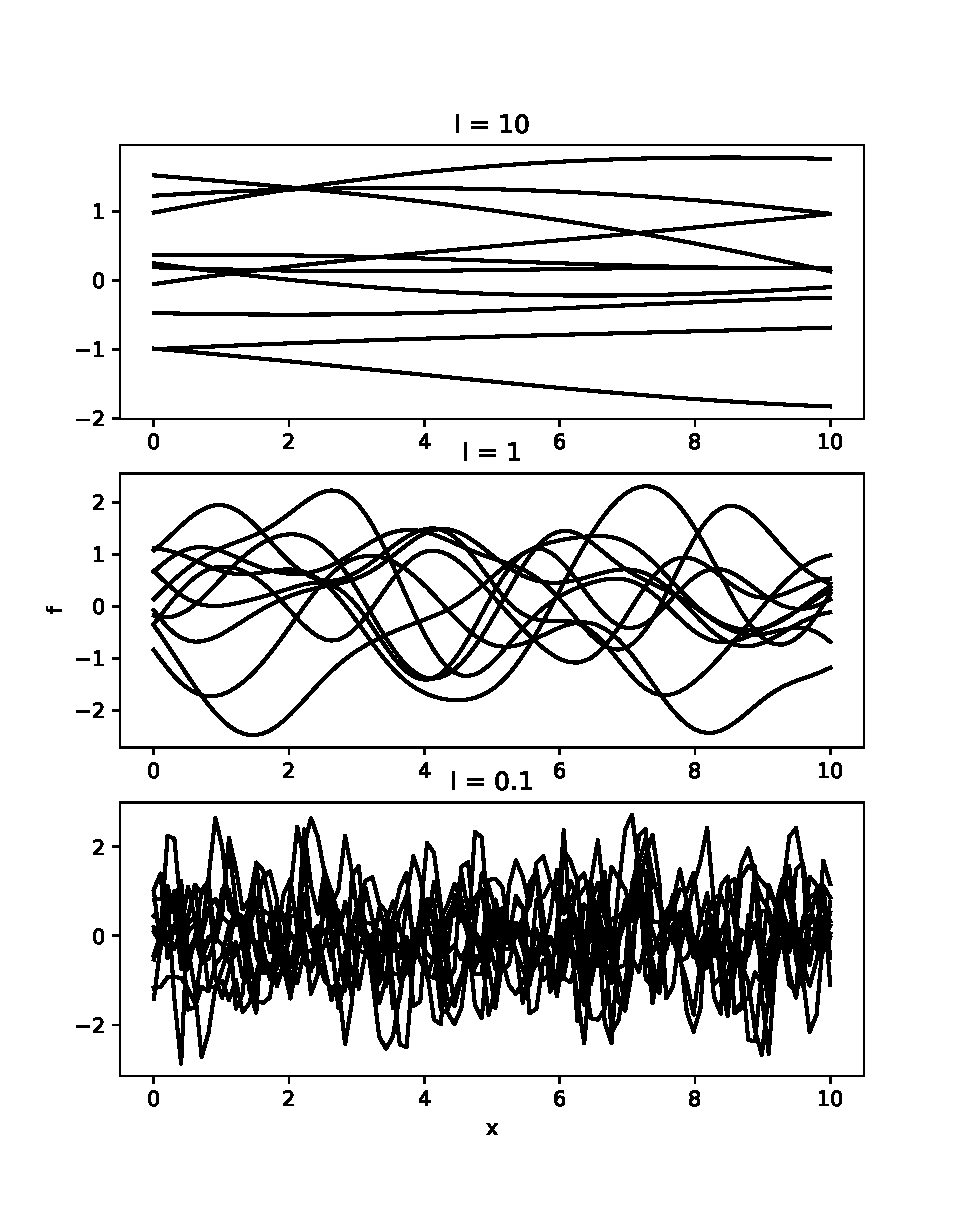
\includegraphics[scale=0.6,trim={0 1cm 0 1cm},clip]{figures/f_prior.pdf}
	\caption{100 samples of $\f \sim \mathcal{N}(\f,\boldsymbol{0},\boldsymbol{K})$, for different values of length scale, $l$.}
	\label{fig:prior_over_f}
\end{figure}
Figure \ref{fig:prior_over_f} shows us that, by increasing the correlation between our inputs, we are inducing \emph{smoothness} in our prior function $f$. As we shall see shortly, `smoothness' is quite an intuitive and useful quantity when it comes to performing regression.\\

%%%%%%%%%%%%%%%%%%%%%%%%%%%%%%%%%%%%%%%%%%%%%%%%%%%%%%%%%%%%%%%%%%%%%%
So, to recap, we have our prior

\begin{equation}
p(\f) = \mathcal{N}(\f;\boldsymbol{0},\boldsymbol{K})
\end{equation}
and we have our noise model, equation (\ref{eq:noise_model}). As we have assumed that the noise affecting our observations is independent for each data point, it follows that

\begin{equation}
	p(\y|\f) = \mathcal{N}\left( \y; \f, \boldsymbol{I}\sigma^2 \right)
\end{equation}
We can then marginalise over $\f$, to find the probability of witnessing $\y$:

\begin{equation}
	p(\y) = \int p(\y|\f)p(\f) d\f
\end{equation}
Fortunately, we can find a closed-from expression for $p(\y)$ using some generic expressions for Gaussian distributions (see Appendix \ref{sec:properties_of_gaussians}). After some manipulation, we find that

\begin{equation}
	p(\y) = \mathcal{N}(\y;\boldsymbol{0},\boldsymbol{C})
	\label{eq:py}
\end{equation}
where

\begin{equation}
	\boldsymbol{C} = \boldsymbol{I}\sigma^2 + \boldsymbol{K} \implies C_{ij} = \sigma^2 \delta_{ij} + k(\boldsymbol{x}_i,\boldsymbol{x}_j).
	\label{eq:C}
\end{equation}
Now, what we really want to do is analyse the probability that, in response to a new input, $\x_*$, we would observe the response $y_*$. Using the relationship we derived in equation (\ref{eq:C}), we can write

\begin{equation}
p(\y,y_*) = \mathcal{N}\left( 
\left(
\begin{array}{c}
	\y \\
	y_* \\
\end{array}
\right);\left(
\begin{array}{c}
	\boldsymbol{0}\\
	0\\
\end{array}\right),	
\left[
  \begin{array}{cc}
    \boldsymbol{C} & \boldsymbol{k} \\
    \boldsymbol{k}^T & c \\
  \end{array}
\right]
 \right)
\end{equation}
where the vector $\boldsymbol{k}$ is defined as

\begin{equation}
	\boldsymbol{k}_n = k(\x_n,\x_*), \qquad n = 1,...,N
\end{equation}
and

\begin{equation}
	c 	= \sigma^2 + k(\x_*,\x_*).
\end{equation}
By once again exploiting our generic expressions for Gaussian distributions, we are then able to find that

\begin{equation}
	p(y_*|\y) = \mathcal{N}(y_*;m_*,\sigma_*^2)
\end{equation}
where

\begin{equation}
	m_* = \boldsymbol{k}^T\boldsymbol{C}^{-1}\boldsymbol{y}, \qquad \sigma_*^2 = c-\boldsymbol{k}^T\boldsymbol{C}^{-1}\boldsymbol{k}.
\end{equation}

%%%%%%%%%%%%%%%%%%%%%%%%%%%%%%%%%%%%%%%%%%%%%%%%%%%%%%%%%%%%%%%%%%%%%%%%
\section{Example: 1D Interpolation}
Here we have generated some `observations' according to:

\begin{equation}
	y_n = \sin x_n + \epsilon, \qquad \epsilon \sim \mathcal{N}(\epsilon;0,\sigma^2)
\end{equation}
where $\sigma = 0.2$. We are going to use a Gaussian process to `fill the gaps' between the data that we have gathered. Using the kernel function in equation (\ref{eq:typical_kernel_function}), Figure \ref{fig:first_regression} shows what happens when we set $l =0.5,1$ and 5 respectively.\\

\begin{figure}[H]
	\centering
	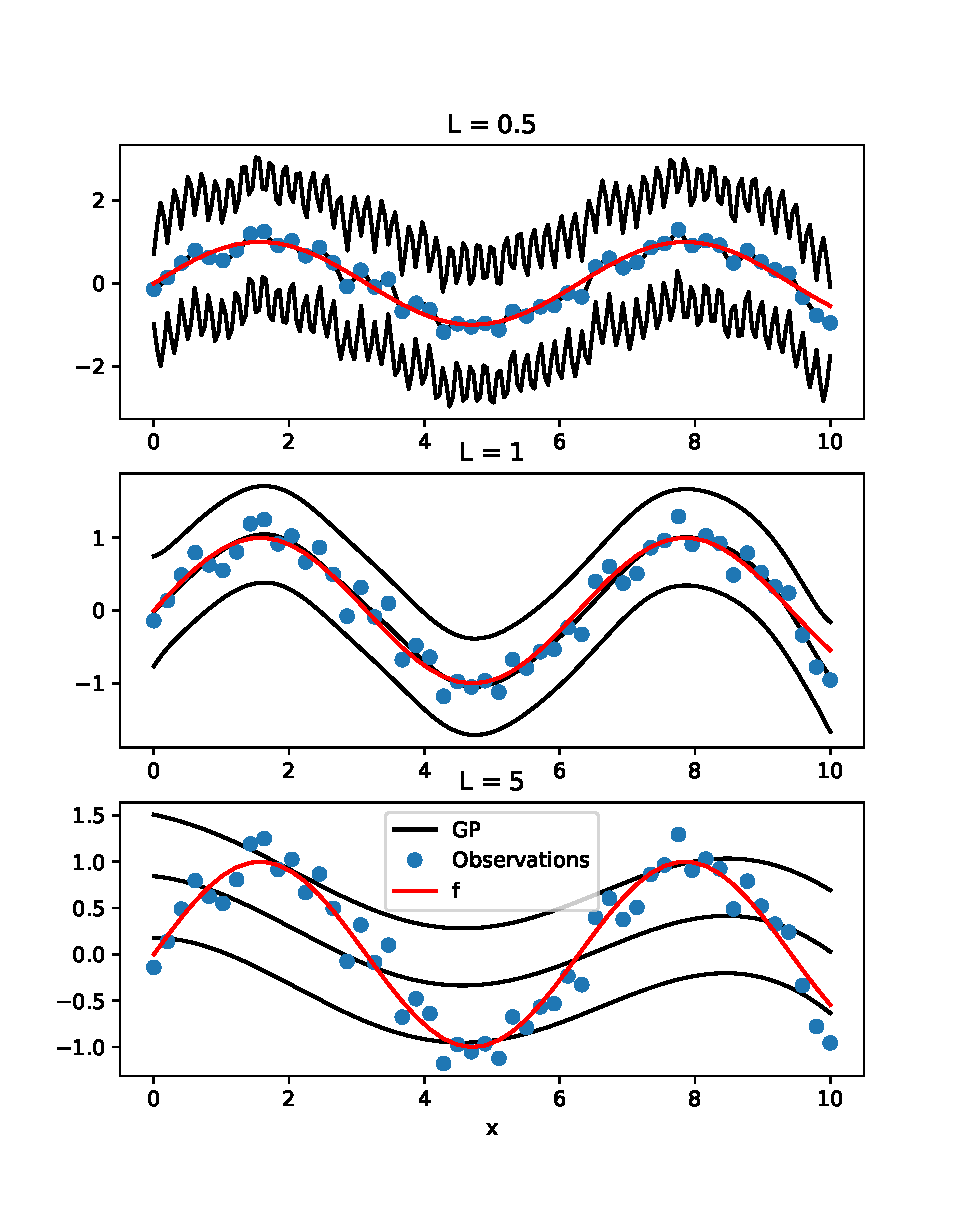
\includegraphics[scale=0.6,trim={0 1cm 0 1cm},clip]{figures/Example1.pdf}
	\caption{Performing Gaussian Process regression for different values of the length scale, $l$. Gaussian Process confidence bounds are 3 standard deviations from the mean.}
	\label{fig:first_regression}
\end{figure}

From Figure \ref{fig:first_regression} it should be obvious that, when $l=0.5$, our interpolating function isn't smooth enough. In fact, it passes through every observation almost exactly - by mistakenly fitting to the noise that is in the data, it has formed a poor representation of the true function, $f$. This phenomenon is sometimes referred to as `overfitting'. When $l=1$, the fit appears sensible while, when $l=5$, our fit seems overly smooth (in other words, it is not able to react quickly enough to changes in the input, $x$). 

%%%%%%%%%%%%%%%%%%%%%%%%%%%%%%%%%%%%%%%%%%%%%%%%%%%%%%%%%%%%%%%%%%%%%%%
\section{Gaussian Process Learning}
A useful aspect of GPs is that, unlike our linear regression approach where we had to begin by assuming a functional form for $f$ (equation (\ref{eq:linear_regression})), GPs are not so tightly constrained. They are sometimes referred to as a form of \emph{non-parametric regression} as they are not limited to only consider one parametric family of regression functions. The GP does, however, have some parameters which require tuning ($l$ and $\sigma$ is our case). These, perhaps a little confusingly, are often referred to as \emph{hyperparameters}.\\ 

Writing our hyperparameters together as $\pa_{\text{hyp}}$ such that $\pa_{\text{hpy}} = \{ l,\sigma \}$ then, from equation (\ref{eq:py}) (derived in the previous section), we know that the probability of witnessing our observations conditional on $\pa_{\text{hyp}}$ is given by

\begin{equation}
	p(\y|\pa_{\text{hyp}}) = \mathcal{N}(\y;\boldsymbol{0},\boldsymbol{C}) = \left((2\pi)^N |\boldsymbol{C}|\right)^{-1/2} \exp\left( -\frac{1}{2} \y^T\boldsymbol{C}^{-1}\y \right)
\end{equation}
such that:

\begin{equation}
	\log p(\y|\pa_{\text{hyp}}) = -\frac{1}{2} \left( N\log 2\pi + \log |\boldsymbol{C}| + \y^T \boldsymbol{C}^{-1} \y  \right).
	\label{eq:log_likelihood}
\end{equation}
Finding the maximum of equation (\ref{eq:log_likelihood}), we can therefore find the maximum likelihood estimates of $\pa_{\text{hyp}}$. This is typically what happens during the `learning process' for a GP. Conveniently, to help our optimisation routine, we are usually able to evaluate the gradient of the log-likelihood with respect to our hyperparameters using closed-form expressions. For example, noting that:

\begin{equation}
	\frac{\partial \log |\boldsymbol{C}|}{\partial \theta_{\text{hyp},i}} = \Tr\left( \boldsymbol{C}^{-1} \frac{\partial \boldsymbol{C}}{\partial \theta_{\text{hyp},i}} \right), \qquad \frac{\partial \boldsymbol{C}^{-1}}{\partial \theta_{\text{hyp},i}} = -\boldsymbol{C}^{-1} \frac{\partial \boldsymbol{C}}{\partial \theta_{\text{hyp},i}} \boldsymbol{C}^{-1}
\end{equation}
then it can be shown that

\begin{equation}
	\frac{\partial}{\partial \theta_{\text{hyp},i}} \log p(\y|\pa_{\text{hyp}}) = -\frac{1}{2} \left( \Tr\left( \boldsymbol{C}^{-1} \frac{\partial \boldsymbol{C}}{\partial \theta_{\text{hyp},i}} \right) - \y^T \boldsymbol{C}^{-1} \frac{\partial \boldsymbol{C}}{\partial \theta_{\text{hyp},i}} \boldsymbol{C}^{-1} \y \right).
\end{equation}	

%%%%%%%%%%%%%%%%%%%%%%%%%%%%%%%%%%%%%%%%%%%%%%%%%%%%%%%%%%%%%%%%%%%%%%%%
\section{Example Python Code}
Code accompanying this tutorial is written in Python (version 2), is heavily commented and is designed to be readable. The module `LIRU\_GP' contains all of the functions needed to train a GP for regression. The scripts `1D\_regression\_example' and `2D\_regression\_example', as the names imply, use LIRU\_GP to perform regression on a 1D and 2D problem respectively. `1D\_regression\_example' will plot results similar to those shown in Figure \ref{fig:1D_regression_example} while `2D\_regression\_example' will produce results similar to those shown in Figure \ref{fig:2D_regression_example}.\\

\begin{figure}[H]
	\centering
	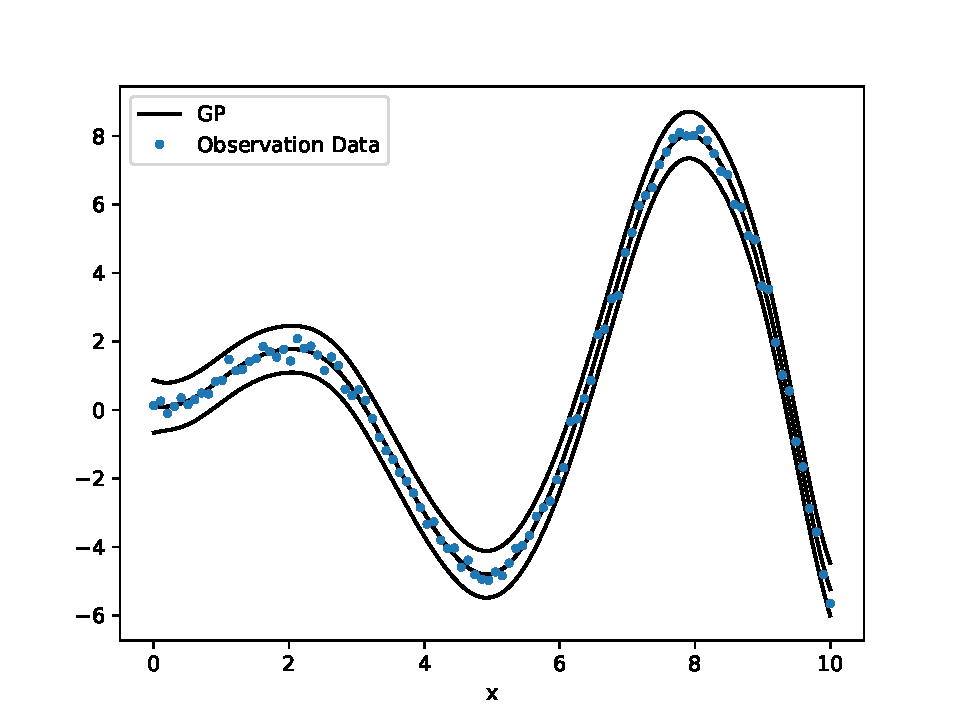
\includegraphics[scale=0.6,trim={0 0cm 0 0cm},clip]{figures/1D_regression.pdf}
	\caption{Example output of `1D\_regression\_example'.}
	\label{fig:1D_regression_example}
\end{figure}

\begin{figure}[H]
	\centering
	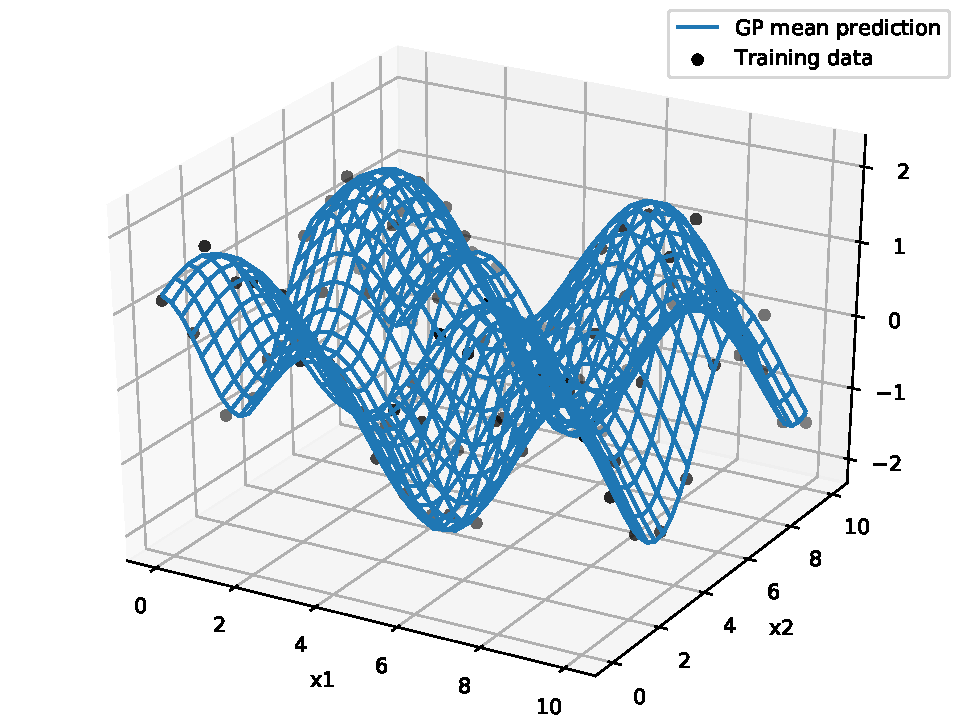
\includegraphics[scale=0.6,trim={0 0cm 0 0cm},clip]{figures/2D_regression.pdf}
	\caption{Example output of `2D\_regression\_example'.}
	\label{fig:2D_regression_example}
\end{figure}

Note that, for more optimised and generic code, a variety of GP packages are offered though Python (see \url{https://sheffieldml.github.io/GPy/} for example) and Matlab (\url{http://www.gaussianprocess.org/gpml/code/matlab/doc/} for example). For a more comprehensive list of available software, see \url{http://gaussianprocess.org/}. As stated previously, the intention here is to provide code that is readable, rather than generic. \\

%%%%%%%%%%%%%%%%%%%%%%%%%%%%%%%%%%%%%%%%%%%%%%%%%%%%%%%%%%%%%%%%%%%%%%%%
%\section{Extrapolation}\label{sec:extrapolation}
%A note on extrapolation - like all data-based methods, GPs cannot be trusted to make predictions at inputs that are far from the available training data. So what does happen if our new input, $\boldsymbol{x}_*$, is far from anything which has been seen before? If $\boldsymbol{x}_*$ really is unlike any of the inputs in the training data then this will be reflected in the vector $\boldsymbol{k}$, whose elements will tend to zero. This means that

%\begin{equation}
%	m_* = \boldsymbol{k}^T\boldsymbol{C}^{-1}\y \rightarrow 0, \qquad \sigma_*^2 = c - \boldsymbol{k}^T\boldsymbol{C}^{-1}\boldsymbol{k} \rightarrow c.
%\end{equation}
%Now, recalling that the prior distribution was $p(\f)=\mathcal{N}(\f;\boldsymbol{0},\boldsymbol{K})$ which led to $p(\y)=\mathcal{N}(\y;\boldsymbol{0},\boldsymbol{C})$, it follows that the prior probability our witnessing $y_*$, is given by

%\begin{equation}
%p(y_*) = \mathcal{N}(y_*;0,c).
%\end{equation}
%Consequently, moving far away from the training data, the GP therefore becomes completely dependent on the prior and not on the information in the data. 



%%%%%%%%%%%%%%%%%%%%%%%%%%%%%%%%%%%%%%%%%%%%%%%%%%%%%%%%%%%%%%%%%%%%%%%%
\newpage
\appendix

\section{Properties of Gaussians}\label{sec:properties_of_gaussians}
Before we start we should note some useful properties. All this stuff if proved in Appendix \ref{sec:Gaussian_proofs} (which is just a slightly longer version of what you can find in Bishop \cite{Bishop2013}). \\

Say we have a partitioned Gaussian $p(\boldsymbol{x}) \propto \exp(-\frac{1}{2}\phi)$ where

\begin{equation}
\phi = \left((\boldsymbol{x}_a-\boldsymbol{\mu}_a)^T, (\boldsymbol{x}_b-\boldsymbol{\mu}_b)^T \right)
\left[\
  \begin{array}{cc}
    \boldsymbol{A}_{aa} & \boldsymbol{A}_{ab} \\
    \boldsymbol{A}_{ba} & \boldsymbol{A}_{bb} \\
  \end{array}
\right]
\left(
  \begin{array}{c}
    \boldsymbol{x}_a-\boldsymbol{\mu}_a \\
    \boldsymbol{x}_b-\boldsymbol{\mu}_b \\
  \end{array}
\right).
\end{equation}

\begin{equation}
= \left((\boldsymbol{x}_a-\boldsymbol{\mu}_a)^T, (\boldsymbol{x}_b-\boldsymbol{\mu}_b)^T \right)
\left[\
  \begin{array}{cc}
    \boldsymbol{\Sigma}_{aa} & \boldsymbol{\Sigma}_{ab} \\
    \boldsymbol{\Sigma}_{ba} & \boldsymbol{\Sigma}_{bb} \\
  \end{array}
\right]^{-1}
\left(
  \begin{array}{c}
    \boldsymbol{x}_a-\boldsymbol{\mu}_a \\
    \boldsymbol{x}_b-\boldsymbol{\mu}_b \\
  \end{array}
\right).
\end{equation}
Written in terms of precision matrices we have the properties that:

\begin{table}[H]
\centering
\begin{tabular}{c|c|c}
  Distribution & Precision & Mean \\
  \hline
  $p(\boldsymbol{x}_a|\boldsymbol{x}_b)$ & $\boldsymbol{A}_{aa}$  & $\boldsymbol{A}^{-1}_{aa} \left( \boldsymbol{A}_{aa} \boldsymbol{\mu}_a - \boldsymbol{A}_{ab}(\boldsymbol{x}_b-\boldsymbol{\mu}_b) \right)$ \\

  $p(\boldsymbol{x}_b|\boldsymbol{x}_a)$ & $\boldsymbol{A}_{bb}$ & $\boldsymbol{A}_{bb}^{-1} \left( \boldsymbol{A}_{bb}\boldsymbol{\mu}_b - \boldsymbol{A}_{ba}(\boldsymbol{x}_a-\boldsymbol{\mu}_a) \right)$ \\

  $p(\boldsymbol{x}_a)$ & $\boldsymbol{A}_{aa} - \boldsymbol{A}_{ab}\boldsymbol{A}_{bb}^{-1} \boldsymbol{A}_{ba}$ & $\boldsymbol{\mu}_a$  \\

  $p(\boldsymbol{x}_b)$ & $\boldsymbol{A}_{bb} - \boldsymbol{A}_{ba}\boldsymbol{A}_{aa}^{-1} \boldsymbol{A}_{ab}$ & $\boldsymbol{\mu}_b$  \\
\end{tabular}
\end{table}
Written in terms of covariance matrices these can also be written as:

\begin{table}[H]
\centering
\begin{tabular}{c|c|c}
  Distribution & Covariance & Mean \\
  \hline
  $p(\boldsymbol{x}_a|\boldsymbol{x}_b)$ & $\boldsymbol{\Sigma}_{aa} - \boldsymbol{\Sigma}_{ab}\boldsymbol{\Sigma}_{bb}^{-1}\boldsymbol{\Sigma}_{ba}$ & $\boldsymbol{\mu}_a + \boldsymbol{\Sigma}_{ab} \boldsymbol{\Sigma}_{bb}^{-1} (\boldsymbol{x}_b-\boldsymbol{\mu}_b)$ \\

  $p(\boldsymbol{x}_b|\boldsymbol{x}_a)$ & $\boldsymbol{\Sigma}_{bb} - \boldsymbol{\Sigma}_{ba}\boldsymbol{\Sigma}_{aa}^{-1}\boldsymbol{\Sigma}_{ab}$ & $\boldsymbol{\mu}_b + \boldsymbol{\Sigma}_{ba} \boldsymbol{\Sigma}_{aa}^{-1} (\boldsymbol{x}_a-\boldsymbol{\mu}_a)$ \\

  $p(\boldsymbol{x}_a)$ & $\boldsymbol{\Sigma}_{aa}$ & $\boldsymbol{\mu}_a$  \\
  $p(\boldsymbol{x}_b)$ & $\boldsymbol{\Sigma}_{bb}$ & $\boldsymbol{\mu}_b$  \\
\end{tabular}
\end{table}
Finally, for the case where

\begin{equation}
p(\boldsymbol{x}_a) = \mathcal{N}(\boldsymbol{\mu},\boldsymbol{A}^{-1}), \qquad p(\boldsymbol{x}_b|\boldsymbol{x}_a) = \mathcal{N}(\boldsymbol{Hx}_a+\boldsymbol{b},\boldsymbol{L}^{-1})
\end{equation}
then we have

\begin{table}[H]
\centering
\begin{tabular}{c|c|c|}
  Distribution & Covariance & Mean \\
  \hline
  $p(\boldsymbol{x}_a|\boldsymbol{x}_b)$ & $( \boldsymbol{A} + \boldsymbol{H}^T\boldsymbol{LH} )^{-1}$ & $( \boldsymbol{A} + \boldsymbol{H}^T\boldsymbol{LH} )^{-1} \left(  \boldsymbol{A\mu} + \boldsymbol{H}^T\boldsymbol{L}(\boldsymbol{x}_b-\boldsymbol{b}) \right)$ \\
  $p(\boldsymbol{x}_b)$ & $\boldsymbol{L}^{-1} + \boldsymbol{HA}^{-1}\boldsymbol{H}^T$ & $\boldsymbol{H\mu}+\boldsymbol{b}$ \\
\end{tabular}
\end{table}
These expressions are generic - they will simplify down a lot for the examples shown here.

%%%%%%%%%%%%%%%%%%%%%%%%%%%%%%%%%%%%%%%%%%%%%%%%%%%%%%%%%%%%%%%%%%%%%%%
\section{Deriving the properties of Gaussian distributions}\label{sec:Gaussian_proofs}
\subsection{Partitioned Gaussian}
We have a Gaussian distribution $p(\boldsymbol{x}) = \exp(-\frac{1}{2}\phi(\boldsymbol{x}))$ where

\begin{equation}
\phi = (\boldsymbol{x}-\boldsymbol{\mu})^T \boldsymbol{A} (\boldsymbol{x}-\boldsymbol{\mu})
\end{equation}
where $\boldsymbol{A}$ is the precision matrix. We are going to partition this up:

\begin{equation}
\boldsymbol{x} = (\boldsymbol{x}_a,\boldsymbol{x}_b )^T, \qquad \boldsymbol{\mu} = ( \boldsymbol{\mu}_a,\boldsymbol{\mu}_b )^T, \qquad \boldsymbol{A} =
\left[\
  \begin{array}{cc}
    \boldsymbol{A}_{aa} & \boldsymbol{A}_{ab} \\
    \boldsymbol{A}_{ba} & \boldsymbol{A}_{bb} \\
  \end{array}
\right]\
\end{equation}
such that $p(\boldsymbol{x}) = p(\boldsymbol{x}_a,\boldsymbol{x}_b) \propto \exp(-\frac{1}{2} \phi)$ where

\begin{equation}
\phi = \left((\boldsymbol{x}_a-\boldsymbol{\mu}_a)^T, (\boldsymbol{x}_b-\boldsymbol{\mu}_b)^T \right)
\left[\
  \begin{array}{cc}
    \boldsymbol{A}_{aa} & \boldsymbol{A}_{ab} \\
    \boldsymbol{A}_{ba} & \boldsymbol{A}_{bb} \\
  \end{array}
\right]\
\left(
  \begin{array}{c}
    \boldsymbol{x}_a-\boldsymbol{\mu}_a \\
    \boldsymbol{x}_b-\boldsymbol{\mu}_b \\
  \end{array}
\right)
\end{equation}

\begin{equation*}
= (\boldsymbol{x}_a-\boldsymbol{\mu}_a)^T \boldsymbol{A}_{aa} (\boldsymbol{x}_a-\boldsymbol{\mu}_a) + (\boldsymbol{x}_a-\boldsymbol{\mu}_a)^T \boldsymbol{A}_{ab} (\boldsymbol{x}_b-\boldsymbol{\mu}_b)
\end{equation*}

\begin{equation}
+ (\boldsymbol{x}_b-\boldsymbol{\mu}_b)^T \boldsymbol{A}_{ba} (\boldsymbol{x}_a-\boldsymbol{\mu}_a) +
(\boldsymbol{x}_b-\boldsymbol{\mu}_b)^T \boldsymbol{A}_{bb} (\boldsymbol{x}_b-\boldsymbol{\mu}_b).
\label{eq:partitioned_Gaussian}
\end{equation}

\subsection{Conditional Gaussian}
We are going to take $p(\boldsymbol{x}_a,\boldsymbol{x}_b)$ and find $p(\boldsymbol{x}_a|\boldsymbol{x}_b)$. This essentially involves taking equation (\ref{eq:partitioned_Gaussian}) and treating all the $\boldsymbol{x}_b$ terms as being constant (which we'll lose when the distribution is normalised). Consequently, defining $C$ as `some constant' and noting that

\begin{equation}
(\boldsymbol{x}_a-\boldsymbol{\mu}_a)^T \boldsymbol{A}_{ab} (\boldsymbol{x}_b-\boldsymbol{\mu}_b) =
(\boldsymbol{x}_b-\boldsymbol{\mu}_b)^T \boldsymbol{A}_{ba} (\boldsymbol{x}_a-\boldsymbol{\mu}_a)
\end{equation}
(as $\boldsymbol{A}_{ab}^T=\boldsymbol{A}_{ba}$) then we find that

\begin{equation}
\phi = (\boldsymbol{x}_a-\boldsymbol{\mu}_a)^T \boldsymbol{A}_{aa} (\boldsymbol{x}_a-\boldsymbol{\mu}_a)
+ 2 (\boldsymbol{x}_a-\boldsymbol{\mu}_a)^T \boldsymbol{A}_{ab} (\boldsymbol{x}_b-\boldsymbol{\mu}_b)  + C
\end{equation}

\begin{equation}
= \boldsymbol{x}_a^T \boldsymbol{A}_{aa} \boldsymbol{x}_a - 2 \boldsymbol{x}_a^T \left( \boldsymbol{A}_{aa} \boldsymbol{\mu}_a - \boldsymbol{A}_{ab}(\boldsymbol{x}_b-\boldsymbol{\mu}_b) \right) + C
\end{equation}
and so, by completing the square, we find that $p(\boldsymbol{x}_a|\boldsymbol{x}_b)$ is Gaussian with precision matrix

\begin{equation}
\boldsymbol{A}_{a|b} = \boldsymbol{A}_{aa}
\end{equation}
and mean

\begin{equation}
\boldsymbol{\mu}_{a|b} = \boldsymbol{A}^{-1}_{aa} \left( \boldsymbol{A}_{aa} \boldsymbol{\mu}_a - \boldsymbol{A}_{ab}(\boldsymbol{x}_b-\boldsymbol{\mu}_b) \right)
\end{equation}

\begin{equation}
= \boldsymbol{\mu}_a - \boldsymbol{A}_{aa}^{-1}\boldsymbol{A}_{ab}(\boldsymbol{x}_b-\boldsymbol{\mu}_b).
\end{equation}
By inverting the precision matrix (which we won't go into here) we can also show that

\begin{equation}
\boldsymbol{\mu}_{a|b} = \boldsymbol{\mu}_a + \boldsymbol{\Sigma}_{ab} \boldsymbol{\Sigma}_{bb}^{-1} (\boldsymbol{x}_b-\boldsymbol{\mu}_b)
\end{equation}

\begin{equation}
\boldsymbol{\Sigma}_{a|b} = \boldsymbol{\Sigma}_{aa} - \boldsymbol{\Sigma}_{ab}\boldsymbol{\Sigma}_{bb}^{-1}\boldsymbol{\Sigma}_{ba}.
\end{equation}
Using the same basic method you can get similar expressions for $p(\boldsymbol{x}_b|\boldsymbol{x}_a)$.

\subsection{Marginalised Gaussian}
Now we will find $p(\boldsymbol{x}_a) = \int p(\boldsymbol{x}_a,\boldsymbol{x}_b) d \boldsymbol{x}_b$. To do this we will collect together all of the $\boldsymbol{x}_b$ terms in equation (\ref{eq:partitioned_Gaussian}) and complete the square. By doing this, when we integrate over $\boldsymbol{x}_b$, we will simply get the normalising constant of a Gaussian which can be absorbed into the constant $C$. We then just collect together all the remaining $\boldsymbol{x}_a$ terms and complete the square again.\\

 To that end, all the terms involving $\boldsymbol{x}_b$ in equation (\ref{eq:partitioned_Gaussian}) are:

\begin{equation}
(\boldsymbol{x}_b-\boldsymbol{\mu}_b)^T \boldsymbol{A}_{bb} (\boldsymbol{x}_b-\boldsymbol{\mu}_b) +
(\boldsymbol{x}_b-\boldsymbol{\mu}_b)^T \boldsymbol{A}_{ba} (\boldsymbol{x}_a-\boldsymbol{\mu}_a)
\end{equation}

\begin{equation}
= \boldsymbol{x}_b^T \boldsymbol{A}_{bb} \boldsymbol{x}_b - 2\boldsymbol{x}_b^T\left( \boldsymbol{A}_{bb}\boldsymbol{\mu}_b - \boldsymbol{A}_{ba}(\boldsymbol{x}_a-\boldsymbol{\mu}_a) \right) + C
\end{equation}

\begin{equation}
= (\boldsymbol{x}_b - \boldsymbol{A}_{bb}^{-1} \boldsymbol{m})^T  \boldsymbol{A}_{bb} (\boldsymbol{x}_b - \boldsymbol{A}_{bb}^{-1} \boldsymbol{m}) - \boldsymbol{m}^T\boldsymbol{A}_{bb}^{-1} \boldsymbol{m} + C
\end{equation}
where

\begin{equation}
\boldsymbol{m} = \boldsymbol{A}_{bb}\boldsymbol{\mu}_b - \boldsymbol{A}_{ba}(\boldsymbol{x}_a-\boldsymbol{\mu}_a).
\end{equation}
Notice we've not included $\boldsymbol{m}^T\boldsymbol{A}_{bb}^{-1} \boldsymbol{m}$ in $C$ as it contains some $\boldsymbol{x}_a$ terms. Once we have integrated over $\boldsymbol{x}_b$ we will be left with the $\boldsymbol{x}_a$ terms left over from equation (\ref{eq:partitioned_Gaussian}) and $-\boldsymbol{m}^T\boldsymbol{A}_{bb}\boldsymbol{m}$. \\

With

\begin{equation}
\boldsymbol{m}^T\boldsymbol{A}_{bb}^{-1} \boldsymbol{m} = \left( \boldsymbol{A}_{bb}\boldsymbol{\mu}_b - \boldsymbol{A}_{ba}(\boldsymbol{x}_a-\boldsymbol{\mu}_a) \right)^T \boldsymbol{A}_{bb}^{-1} \left( \boldsymbol{A}_{bb}\boldsymbol{\mu}_b - \boldsymbol{A}_{ba}(\boldsymbol{x}_a-\boldsymbol{\mu}_a) \right)
\end{equation}

\begin{equation}
\boldsymbol{x}_a^T \boldsymbol{A}_{ab} \boldsymbol{A}_{bb}^{-1} \boldsymbol{A}_{ba} \boldsymbol{x}_a - 2\boldsymbol{x}_a^T ( \boldsymbol{A}_{ab}\boldsymbol{\mu}_b + \boldsymbol{A}_{ab}\boldsymbol{A}_{bb}^{-1} \boldsymbol{A}_{ba} \boldsymbol{\mu}_a ) + C
\end{equation}
and, as we have

\begin{equation}
\boldsymbol{x}_a^T \boldsymbol{A}_{aa} \boldsymbol{x}_a - 2\boldsymbol{x}_a^T \boldsymbol{A}_{aa} \boldsymbol{\mu}_a - 2\boldsymbol{x}_a^T \boldsymbol{A}_{ab}\boldsymbol{\mu}_b + C
\end{equation}
from the left over $\boldsymbol{x}_a$ terms, it follows that after integrating out $\boldsymbol{x}_b$ we are left with

\begin{equation}
\boldsymbol{x}_a^T (\boldsymbol{A}_{aa} - \boldsymbol{A}_{ab}\boldsymbol{A}_{bb}^{-1}\boldsymbol{A}_{ba}  )\boldsymbol{x}_a - 2\boldsymbol{x}_a( \boldsymbol{A}_{aa} - \boldsymbol{A}_{ab}\boldsymbol{A}_{bb}^{-1}\boldsymbol{A}_{ba} ) \boldsymbol{\mu}_a + C.
\end{equation}
Consequently, $p(\boldsymbol{x}_a) = \int p(\boldsymbol{x}_a,\boldsymbol{x}_b) d\boldsymbol{x}_b$ has precision matrix

\begin{equation}
\boldsymbol{A}_a = \boldsymbol{A}_{aa} - \boldsymbol{A}_{ab}\boldsymbol{A}_{bb}^{-1} \boldsymbol{A}_{ba}
\end{equation}
and mean

\begin{equation}
\boldsymbol{A}_a^{-1} (  \boldsymbol{A}_{aa} - \boldsymbol{A}_{ab}\boldsymbol{A}_{bb}^{-1} \boldsymbol{A}_{ba} ) \boldsymbol{\mu}_a = \boldsymbol{\mu}_a
\end{equation}
which is nice. Furthermore, taking the inverse of the precision matrix (which we won't do here) we find that

\begin{equation}
\boldsymbol{\Sigma}_a = \boldsymbol{\Sigma}_{aa}
\end{equation}
which is also nice.

\subsection{Bayes' theorem for a linear Gaussian model}
Say we have

\begin{equation}
p(\boldsymbol{x}_a) = \mathcal{N}(\mu,\boldsymbol{A}^{-1}), \qquad p(\boldsymbol{x}_b|\boldsymbol{x}_a) = \mathcal{N}(\boldsymbol{Hx}_a+\boldsymbol{b},\boldsymbol{L}^{-1})
\end{equation}
and we wish to evaluate Bayes' theorem:

\begin{equation}
p(\boldsymbol{x}_a|\boldsymbol{x}_b) \propto p(\boldsymbol{x}_b|\boldsymbol{x}_a)p(\boldsymbol{x}_a).
\end{equation}
The easiest way to do is actually to write an expression for $p(\boldsymbol{x}_a,\boldsymbol{x}_b)$ before finding $p(\boldsymbol{x}_a|\boldsymbol{x}_b)$ using the stuff we derived earlier. To that end, writing $\boldsymbol{z}^T = (\boldsymbol{x}_1^T,\boldsymbol{x}_2^T)$ then we have $p(\boldsymbol{z})\propto \exp(-\frac{1}{2} \phi)$ where

\begin{equation}
\phi = (\boldsymbol{x}_a-\boldsymbol{\mu})^T \boldsymbol{A} (\boldsymbol{x}_a-\boldsymbol{\mu}) + (\boldsymbol{x}_b-\boldsymbol{Hx}_a-\boldsymbol{b})^T \boldsymbol{L} (\boldsymbol{x}_b-\boldsymbol{Hx}_a-\boldsymbol{b}).
\end{equation}
Collecting together all the second order terms we get

\begin{equation}
\boldsymbol{x}_a^T\boldsymbol{Ax}_a + \boldsymbol{x}_b^T\boldsymbol{Lx}_b - 2\boldsymbol{x}_a^T\boldsymbol{H}^T\boldsymbol{Lx}_b + \boldsymbol{x}_a^T\boldsymbol{H}^T\boldsymbol{LHx}_a
\end{equation}

\begin{equation}
= \left(
    \begin{array}{cc}
      \boldsymbol{x}_a^T & \boldsymbol{x}_b^T \\
    \end{array}
  \right)
  \left[
    \begin{array}{cc}
      \boldsymbol{A} + \boldsymbol{H}^T\boldsymbol{LH} & -\boldsymbol{H}^T\boldsymbol{L} \\
      -\boldsymbol{L}\boldsymbol{H}^T & \boldsymbol{L} \\
    \end{array}
  \right]
  \left(
    \begin{array}{c}
      \boldsymbol{x}_a \\
      \boldsymbol{x}_b \\
    \end{array}
  \right)
\end{equation}
and so $\boldsymbol{z}$ has precision matrix

\begin{equation}
\boldsymbol{R} =  \left[
    \begin{array}{cc}
      \boldsymbol{A} + \boldsymbol{H}^T\boldsymbol{LH} & -\boldsymbol{H}^T\boldsymbol{L} \\
      -\boldsymbol{L}\boldsymbol{H}^T & \boldsymbol{L} \\
    \end{array}
  \right]
\end{equation}
and, it can be shown, covariance matrix

\begin{equation}
\boldsymbol{R}^{-1} =
\left[
  \begin{array}{cc}
    \boldsymbol{A}^{-1} & \boldsymbol{A}^{-1}\boldsymbol{H}^T \\
    \boldsymbol{H}\boldsymbol{A}^{-1} & \boldsymbol{L}^{-1}+\boldsymbol{HA}^{-1}\boldsymbol{H}^T \\
  \end{array}
\right].
\end{equation}
Collecting the first order terms:

\begin{equation}
-2\boldsymbol{x}_a^T\boldsymbol{A\mu} - 2\boldsymbol{x}_b^T\boldsymbol{Lb} + 2\boldsymbol{x}_a^T\boldsymbol{H}^T\boldsymbol{Lb}
\end{equation}

\begin{equation}
= -2 \left(
       \begin{array}{cc}
         \boldsymbol{x}_a^T & \boldsymbol{x}_b^T \\
       \end{array}
     \right)
     \left(
       \begin{array}{c}
         \boldsymbol{A\mu}-\boldsymbol{H}^T\boldsymbol{Lb} \\
         \boldsymbol{Lb} \\
       \end{array}
     \right)
\end{equation}
and so

\begin{equation}
\E[\boldsymbol{z}] = \boldsymbol{R}^{-1}
     \left(
       \begin{array}{c}
         \boldsymbol{A\mu}-\boldsymbol{H}^T\boldsymbol{Lb} \\
         \boldsymbol{Lb} \\
       \end{array}
     \right)
\end{equation}

\begin{equation}
= \left[
  \begin{array}{cc}
    \boldsymbol{A}^{-1} & \boldsymbol{A}^{-1}\boldsymbol{H}^T \\
    \boldsymbol{H}\boldsymbol{A}^{-1} & \boldsymbol{L}^{-1}+\boldsymbol{HA}^{-1}\boldsymbol{H}^T \\
  \end{array}
\right]
     \left(
       \begin{array}{c}
         \boldsymbol{A\mu}-\boldsymbol{H}^T\boldsymbol{Lb} \\
         \boldsymbol{Lb} \\
       \end{array}
     \right) =
     \left(
       \begin{array}{c}
         \boldsymbol{\mu} \\
         \boldsymbol{H\mu} + \boldsymbol{b} \\
       \end{array}
     \right).
\end{equation}
From our expressions for marginalised Gaussians it is clear that

\begin{equation}
p(\boldsymbol{x}_b) = \mathcal{N}(\boldsymbol{H\mu}+\boldsymbol{b}, \boldsymbol{L}^{-1} + \boldsymbol{HA}^{-1}\boldsymbol{H}^T).
\end{equation}
Now, making the substitutions

\begin{equation}
\boldsymbol{A}_{aa} \equiv \boldsymbol{A} + \boldsymbol{H}^T\boldsymbol{LH}, \quad \boldsymbol{\mu}_a \equiv \boldsymbol{\mu}, \quad \boldsymbol{\mu}_b \equiv \boldsymbol{H\mu} + \boldsymbol{b}, \quad \boldsymbol{A}_{ab} \equiv -\boldsymbol{H}^T\boldsymbol{L}
\end{equation}
we can use our expressions for the conditional Gaussian to find $p(\boldsymbol{x}_a|\boldsymbol{x}_b)$. Firstly, note that the posterior precision matrix is

\begin{equation}
\boldsymbol{A} + \boldsymbol{H}^T\boldsymbol{LH}.
\end{equation}
Secondly, as

\begin{equation}
(\boldsymbol{A}+\boldsymbol{H}^T\boldsymbol{LH})\boldsymbol{\mu} + \boldsymbol{H}^T\boldsymbol{L}(\boldsymbol{x}_b-\boldsymbol{H\mu} - \boldsymbol{b}) = \boldsymbol{A\mu} + \boldsymbol{H}^T\boldsymbol{L}(\boldsymbol{x}_b-\boldsymbol{b})
\end{equation}
then mean is

\begin{equation}
( \boldsymbol{A} + \boldsymbol{H}^T\boldsymbol{LH} )^{-1} \left(  \boldsymbol{A\mu} + \boldsymbol{H}^T\boldsymbol{L}(\boldsymbol{x}_b-\boldsymbol{b}) \right).
\end{equation}



\bibliography{bibliography}
\bibliographystyle{unsrt}

\end{document} 
